% Options for packages loaded elsewhere
\PassOptionsToPackage{unicode}{hyperref}
\PassOptionsToPackage{hyphens}{url}
%
\documentclass[
  12pt,a4paper,lualatex,ja=standard]{bxjsarticle}
\usepackage{lmodern}
\usepackage{amsmath}
\usepackage{ifxetex,ifluatex}
\ifnum 0\ifxetex 1\fi\ifluatex 1\fi=0 % if pdftex
  \usepackage[T1]{fontenc}
  \usepackage[utf8]{inputenc}
  \usepackage{textcomp} % provide euro and other symbols
  \usepackage{amssymb}
\else % if luatex or xetex
  \usepackage{unicode-math}
  \defaultfontfeatures{Scale=MatchLowercase}
  \defaultfontfeatures[\rmfamily]{Ligatures=TeX,Scale=1}
\fi
% Use upquote if available, for straight quotes in verbatim environments
\IfFileExists{upquote.sty}{\usepackage{upquote}}{}
\IfFileExists{microtype.sty}{% use microtype if available
  \usepackage[]{microtype}
  \UseMicrotypeSet[protrusion]{basicmath} % disable protrusion for tt fonts
}{}
\makeatletter
\@ifundefined{KOMAClassName}{% if non-KOMA class
  \IfFileExists{parskip.sty}{%
    \usepackage{parskip}
  }{% else
    \setlength{\parindent}{0pt}
    \setlength{\parskip}{6pt plus 2pt minus 1pt}}
}{% if KOMA class
  \KOMAoptions{parskip=half}}
\makeatother
\usepackage{xcolor}
\IfFileExists{xurl.sty}{\usepackage{xurl}}{} % add URL line breaks if available
\IfFileExists{bookmark.sty}{\usepackage{bookmark}}{\usepackage{hyperref}}
\hypersetup{
  hidelinks,
  pdfcreator={LaTeX via pandoc}}
\urlstyle{same} % disable monospaced font for URLs
\usepackage{graphicx}
\makeatletter
\def\maxwidth{\ifdim\Gin@nat@width>\linewidth\linewidth\else\Gin@nat@width\fi}
\def\maxheight{\ifdim\Gin@nat@height>\textheight\textheight\else\Gin@nat@height\fi}
\makeatother
% Scale images if necessary, so that they will not overflow the page
% margins by default, and it is still possible to overwrite the defaults
% using explicit options in \includegraphics[width, height, ...]{}
\setkeys{Gin}{width=\maxwidth,height=\maxheight,keepaspectratio}
% Set default figure placement to htbp
\makeatletter
\def\fps@figure{htbp}
\makeatother
\setlength{\emergencystretch}{3em} % prevent overfull lines
\providecommand{\tightlist}{%
  \setlength{\itemsep}{0pt}\setlength{\parskip}{0pt}}
\setcounter{secnumdepth}{5}
\usepackage{indentfirst}
\parindent = 1em
\usepackage{dcolumn}
\newcolumntype{.}{D{.}{.}{-1}}
\usepackage{caption}
\captionsetup[table]{name=表}
\captionsetup[figure]{name=図}
\usepackage{hyperref}
\pagestyle{empty}
\usepackage{multicol}
\usepackage{ascmac}
\setpagelayout*{top=10truemm,bottom=30truemm,left=10truemm,right=10truemm}
\usepackage{tikz}
\usetikzlibrary{arrows.meta,decorations,decorations.pathreplacing}
\usepackage{tabstackengine}
\usepackage{xcolor}
\usepackage{rotating}
\usepackage{txfonts}
\usepackage{fancybox}
\usepackage{dashbox}
\usepackage{tcolorbox}
\tcbuselibrary{theorems,skins}
\usepackage{siunitx}
\usepackage{framed}
\usepackage{enumerate}
\usepackage{lastpage}
\ifluatex
  \usepackage{selnolig}  % disable illegal ligatures
\fi

\author{}
\date{\vspace{-2.5em}}

\begin{document}

\renewcommand{\thefootnote}{}
\newcounter{kaunta}
\renewcommand{\thekaunta}{\arabic{kaunta}}
\newcommand{\kaunta}{\refstepcounter{kaunta}%
\thekaunta}
\def\question{\noindent\fbox{\large\makebox[1em]{\text{\kaunta}}} \hspace{1pt}}
\newcounter{skaunta}
\renewcommand{\theskaunta}{\arabic{skaunta}}
\newcommand{\skaunta}{\refstepcounter{skaunta}%
\theskaunta}
\def\squestion{(\text{\skaunta})\hspace{2.5pt}}
\newcommand{\maru}[1]{\raise0.2ex\hbox{\textcircled{\scriptsize{#1}}}}
\newcommand{\jsim}{\mathrel{\text{∽}}}
\newcommand{\jpara}{/\!/}

\newcounter{kcounter}
\setcounter{kcounter}{0}
\newcommand{\kana}{\refstepcounter{kcounter}\ifthenelse{\value{kcounter}=1}{ア}{\ifthenelse{\value{kcounter}=2}{イ}{\ifthenelse{\value{kcounter}=3}{ウ}{\ifthenelse{\value{kcounter}=4}{エ}{\ifthenelse{\value{kcounter}=5}{オ} {\ifthenelse{\value{kcounter}=6}{カ}{\ifthenelse{\value{kcounter}=7}{キ}{\ifthenelse{\value{kcounter}=8}{ク}{\ifthenelse{\value{kcounter}=9}{ケ}{\ifthenelse{\value{kcounter}=10}{コ}{\ifthenelse{\value{kcounter}=11}{サ}{\ifthenelse{\value{kcounter}=12}{シ}{\ifthenelse{\value{kcounter}=13}{ス}{\ifthenelse{\value{kcounter}=14}{セ}{\ifthenelse{\value{kcounter}=15}{ソ}{\ifthenelse{\value{kcounter}=16}{タ}{\ifthenelse{\value{kcounter}=17}{チ}{\ifthenelse{\value{kcounter}=18}{ツ}{\ifthenelse{\value{kcounter}=19}{テ}{\ifthenelse{\value{kcounter}=20}{ト}{\ifthenelse{\value{kcounter}=21}{ナ}{\ifthenelse{\value{kcounter}=22}{二}{\ifthenelse{\value{kcounter}=23}{ヌ}{\ifthenelse{\value{kcounter}=24}{ネ}{\ifthenelse{\value{kcounter}=25}{ノ}{\ifthenelse{\value{kcounter}=26}{ハ}{\ifthenelse{\value{kcounter}=27}{ヒ}{\ifthenelse{\value{kcounter}=28}{フ}{\ifthenelse{\value{kcounter}=29}{ヘ}{\ifthenelse{\value{kcounter}=30}{ホ}{\ifthenelse{\value{kcounter}=31}{マ}{\ifthenelse{\value{kcounter}=32}{ミ}{\ifthenelse{\value{kcounter}=33}{ム}{\ifthenelse{\value{kcounter}=34}{メ}{\ifthenelse{\value{kcounter}=35}{モ}{\ifthenelse{\value{kcounter}=36}{ヤ}{\ifthenelse{\value{kcounter}=37}{ユ}{\ifthenelse{\value{kcounter}=38}{ヨ}{\ifthenelse{\value{kcounter}=39}{ラ}{\ifthenelse{\value{kcounter}=40}{リ}{\ifthenelse{\value{kcounter}=41}{ル}{\ifthenelse{\value{kcounter}=42}{レ}{\ifthenelse{\value{kcounter}=43}{ロ}{\ifthenelse{\value{kcounter}=44}{ワ}{・}}}}}}}}}}}}}}}}}}}}}}}}}}}}}}}}}}}}}}}}}}}}}

\newcommand{\kuran}[1]{\framebox[1.5cm][c]{\maru{#1}}}

\newcommand{\haiten}[1]{%
\begin{flushright}%
\footnotesize{<#1>}%
\end{flushright}%
}

\newgeometry{top=10truemm,bottom=10truemm,left=20truemm,right=20truemm}

\thispagestyle{empty}
\begin{center}
\phantom{empty}

\vspace{60truemm}

\hspace{4em} {\HUGE\gtfamily\bfseries 数\hspace{2em}学}\hspace{1em}{\large \gtfamily \bfseries ($\mathbf{1}$年)}\\
\vspace{84truemm}

{\large\gtfamily\bfseries 注\hspace{5em}意}

\end{center}

\centering
\begin{framed}
\begin{flushleft}
\begin{enumerate}[\Large \gtfamily 1]
  \item {\large 「開始」の合図があるまでは,開いてはいけません。}

  \item {\large 問題は\pageref{LastPage}ページまであります。}

  \item {\large 「開始」の合図があったら,まず,問題用紙・解答用紙に,組・番号と名前などを書きなさい。}

  \item {\large 答えは,すべて解答用紙に書きなさい。また、所定の欄に濃くはっきりと書きなさい。}

  \item {\large 「終了」の合図で,すぐ鉛筆をおき,解答用紙を裏返しにしなさい。}
\end{enumerate}
\end{flushleft}
\end{framed}

\vspace{14mm}

\begin{center}
{\large \underline{\hspace{30mm}組 \hspace{30mm}番 \hspace{15mm} 名前 \hspace{60mm}}}
\end{center}

\newpage

\pagestyle{plain}
\pagenumbering{arabic}

\begin{flushleft}

\noindent\fbox{\large\makebox[1em]{\text{\refstepcounter{kaunta}%
\arabic{kaunta}}}} \hspace{1pt}次の空欄にあてはまる語句を下の語群から選びなさい。

%
\begin{flushright}%
\footnotesize{<知・技$2 \times 12$点>}%
\end{flushright}%


いろいろな値をとる文字のことを\framebox[1.5cm][c]{\raise 0.2ex\hbox{\textcircled{\scriptsize{ア}}}}という。\framebox[1.5cm][c]{\raise 0.2ex\hbox{\textcircled{\scriptsize{ア}}}}のとりうる値の範囲を、その\framebox[1.5cm][c]{\raise 0.2ex\hbox{\textcircled{\scriptsize{ア}}}}の\framebox[1.5cm][c]{\raise 0.2ex\hbox{\textcircled{\scriptsize{イ}}}}という。ある\framebox[1.5cm][c]{\raise 0.2ex\hbox{\textcircled{\scriptsize{ア}}}}$x, \, y$があって、\framebox[1.5cm][c]{\raise 0.2ex\hbox{\textcircled{\scriptsize{ア}}}}$x$の値を決めると、それにともなって\framebox[1.5cm][c]{\raise 0.2ex\hbox{\textcircled{\scriptsize{ア}}}}$y$の値もただ1つ決まるとき、$y$は$x$の\framebox[1.5cm][c]{\raise 0.2ex\hbox{\textcircled{\scriptsize{ウ}}}}であるという。

\begin{multicols}{2}
負の数も含めてグラフをかくには、右の図のような、それぞれの原点で直角に交わっている2つの数直線を考えればよい。このような図で、横の数直線を\framebox[1.5cm][c]{\raise 0.2ex\hbox{\textcircled{\scriptsize{エ}}}}、または、横軸、縦の数直線を\framebox[1.5cm][c]{\raise 0.2ex\hbox{\textcircled{\scriptsize{オ}}}}、または、縦軸という。横軸と縦軸を合わせて\framebox[1.5cm][c]{\raise 0.2ex\hbox{\textcircled{\scriptsize{カ}}}}、その交点Oを\framebox[1.5cm][c]{\raise 0.2ex\hbox{\textcircled{\scriptsize{キ}}}}という。

\columnbreak

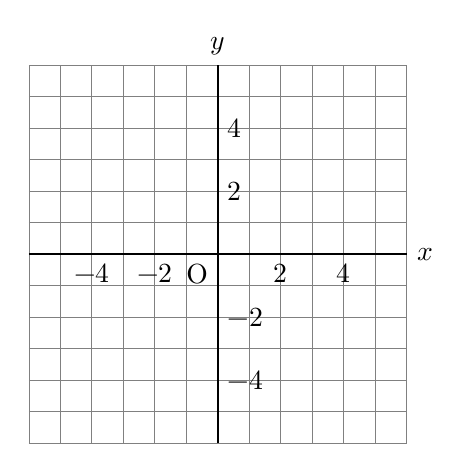
\begin{tikzpicture}[scale=0.4]
\draw[help lines] (-6,-6) grid (6,6);
\draw[thick](-6,0) -- (6,0)node[right]{$x$};
\draw[thick](0,-6) -- (0,6)node[above]{$y$};
\draw(0,0) node[below left]{O};
\foreach \x in {-4, -2, 2, 4} \draw ({\x},0) node[below]{$\x$};
\foreach \y in {-4, -2, 2, 4} \draw (0,{\y}) node[right]{$\y$};
\end{tikzpicture}

\end{multicols}

$y$が$x$の\framebox[1.5cm][c]{\raise 0.2ex\hbox{\textcircled{\scriptsize{ウ}}}}で、次のような式で表されるとき、$y$は$x$に\framebox[1.5cm][c]{\raise 0.2ex\hbox{\textcircled{\scriptsize{ク}}}}するという。

$$
y = ax
$$

一定の数やそれを表す文字を定数といい、上の式のなかの文字$a$は定数であり、\framebox[1.5cm][c]{\raise 0.2ex\hbox{\textcircled{\scriptsize{ケ}}}}という。$y$が$x$に\framebox[1.5cm][c]{\raise 0.2ex\hbox{\textcircled{\scriptsize{ク}}}}し、$x \neq 0$のとき、$\dfrac{y}{x}$の値は一定で、\framebox[1.5cm][c]{\raise 0.2ex\hbox{\textcircled{\scriptsize{ケ}}}}に等しい。

\framebox[1.5cm][c]{\raise 0.2ex\hbox{\textcircled{\scriptsize{ク}}}}のグラフは原点を通る\framebox[1.5cm][c]{\raise 0.2ex\hbox{\textcircled{\scriptsize{コ}}}}となる。

また、$y$が$x$の\framebox[1.5cm][c]{\raise 0.2ex\hbox{\textcircled{\scriptsize{ウ}}}}で、次のような式で表されるとき、$y$は$x$に\framebox[1.5cm][c]{\raise 0.2ex\hbox{\textcircled{\scriptsize{サ}}}}するという。

$$
y = \dfrac{a}{x}
$$
\framebox[1.5cm][c]{\raise 0.2ex\hbox{\textcircled{\scriptsize{サ}}}}についても、定数$a$を\framebox[1.5cm][c]{\raise 0.2ex\hbox{\textcircled{\scriptsize{ケ}}}}という。$y$が$x$に\framebox[1.5cm][c]{\raise 0.2ex\hbox{\textcircled{\scriptsize{サ}}}}するとき、$x$と$y$の積$xy$は一定で、\framebox[1.5cm][c]{\raise 0.2ex\hbox{\textcircled{\scriptsize{ケ}}}}に等しい。

\framebox[1.5cm][c]{\raise 0.2ex\hbox{\textcircled{\scriptsize{サ}}}}のグラフはなめらかな2つの曲線になり、\framebox[1.5cm][c]{\raise 0.2ex\hbox{\textcircled{\scriptsize{シ}}}}とよばれる。このグラフは縦軸、横軸と交わらない。

\begin{itembox}[l]{語群}
係数\hspace{1.5em}項\hspace{1.5em}原点\hspace{1.5em}比例\hspace{1.5em}凡例\hspace{1.5em}変数\hspace{1.5em}定数\hspace{1.5em}反比例\hspace{1.5em}関数\hspace{1.5em}間数\hspace{1.5em}$v$軸\hspace{1.5em}$x$軸\hspace{1.5em}$y$軸\hspace{1.5em} $z$軸\hspace{1.5em}変域\hspace{1.5em}凡例定数\hspace{1.5em}比例定数\hspace{1.5em}曲線\hspace{1.5em}半直線\hspace{1.5em}線分\hspace{1.5em}直線\hspace{1.5em}二曲線\hspace{1.5em}双曲線\hspace{1.5em}縦軸\hspace{1.5em}横軸\hspace{1.5em}絶対値\hspace{1.5em}座標軸
\end{itembox}



\newpage

\noindent\fbox{\large\makebox[1em]{\text{\refstepcounter{kaunta}%
\arabic{kaunta}}}} \hspace{1pt}次のような$x$と$y$の関係について、$y$は$x$の関数であるものを選びなさい。

%
\begin{flushright}%
\footnotesize{<知・技2点>}%
\end{flushright}%


ア\hspace{1em} $x$歳の人の体重は$y\si{kg}$である。

イ\hspace{1em} 半径が$x \si{cm}$の円の面積を$y \si{cm}^2$とする。

ウ\hspace{1em} 縦の長さが$x \si{cm}$の長方形の面積を$y \si{cm}^2$とする。

\vfill

\noindent\fbox{\large\makebox[1em]{\text{\refstepcounter{kaunta}%
\arabic{kaunta}}}} \hspace{1pt}変数$x$が次の値の範囲をとるとき、$x$の変域を不等号を使って表しなさい。

%
\begin{flushright}%
\footnotesize{<知・技$2\times 4$点>}%
\end{flushright}%


(\text{\refstepcounter{skaunta}%
\arabic{skaunta}})\hspace{2.5pt}1より大きく、4以下

(\text{\refstepcounter{skaunta}%
\arabic{skaunta}})\hspace{2.5pt}2未満

(\text{\refstepcounter{skaunta}%
\arabic{skaunta}})\hspace{2.5pt}$-3$より大きい

(\text{\refstepcounter{skaunta}%
\arabic{skaunta}})\hspace{2.5pt}$-1$以上$3$以下

\setcounter{skaunta}{0}

\vfill

\begin{multicols}{2}
\noindent\fbox{\large\makebox[1em]{\text{\refstepcounter{kaunta}%
\arabic{kaunta}}}} \hspace{1pt}右の図で、点A, B, C, Dの座標を答えなさい。また、次の点E, F, Gを解答欄に示しなさい。

%
\begin{flushright}%
\footnotesize{<知・技$2\times 7$点>}%
\end{flushright}%


E$(5, \, 4)$ 

F$(3, \, 0)$

G$(-3, \, 2)$

\columnbreak

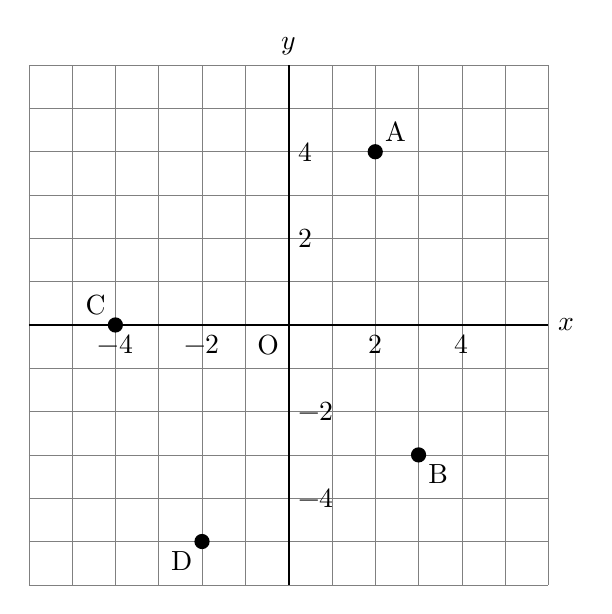
\begin{tikzpicture}[scale=0.55]
\draw[help lines] (-6,-6) grid (6,6);
\draw[thick](-6,0) -- (6,0)node[right]{$x$};
\draw[thick](0,-6) -- (0,6)node[above]{$y$};
\draw (0,0) node[below left]{O};
\foreach \x in {-4, -2, 2, 4} \draw ({\x},0) node[below]{$\x$};
\foreach \y in {-4, -2, 2, 4} \draw (0,{\y}) node[right]{$\y$};
\fill (2, 4) circle[radius=5pt] node[above right]{A};
\fill (3, -3) circle[radius=5pt] node[below right]{B};
\fill (-4, 0) circle[radius=5pt] node[above left]{C};
\fill (-2, -5) circle[radius=5pt] node[below left]{D};
\end{tikzpicture}

\end{multicols}

\vfill

\newpage

\noindent\fbox{\large\makebox[1em]{\text{\refstepcounter{kaunta}%
\arabic{kaunta}}}} \hspace{1pt}次のア〜ウについて、$y$が$x$に比例するものと、反比例するものを選び、記号で答えなさい。また、式も答えなさい。

%
\begin{flushright}%
\footnotesize{<知・技6点>}%
\end{flushright}%


ア\hspace{1em}100kmの道のりを時速$x$kmで走ると、$y$時間かかる。

イ\hspace{1em}200ページの本を$x$ページ読んだときの残りのページ数は$y$ページである。

ウ\hspace{1em}底辺が4cm、高さが$x$cmの三角形の面積は$y$$\si{cm}^2$である。

\vfill

\noindent\fbox{\large\makebox[1em]{\text{\refstepcounter{kaunta}%
\arabic{kaunta}}}} \hspace{1pt}$y$は$x$に比例し、$x = 3$のとき、$y = -9$です。このとき、次の問に答えなさい。

%
\begin{flushright}%
\footnotesize{<知・技(1),(3),(4)2点、(2)4点>}%
\end{flushright}%


(\text{\refstepcounter{skaunta}%
\arabic{skaunta}})\hspace{2.5pt}$y$を$x$の式で表しなさい。

(\text{\refstepcounter{skaunta}%
\arabic{skaunta}})\hspace{2.5pt}次の表を完成させなさい。
\begin{center}
\begin{tabular}{c|ccccccc}
\hline
$x$ & $\cdots$ & $-4$ & $0$ & $4$ & $\cdots$ & $12$ & $\cdots$ \\
\hline
$y$ & $\cdots$ &  &  &  & $\cdots$ & & $\cdots$ \\
\hline
\end{tabular}
\end{center}


(\text{\refstepcounter{skaunta}%
\arabic{skaunta}})\hspace{2.5pt}$x = 2$のときの$y$の値を求めなさい。

(\text{\refstepcounter{skaunta}%
\arabic{skaunta}})\hspace{2.5pt}$x$の値が増加すると、$y$の値は増加しますか、それとも減少しますか。

\setcounter{skaunta}{0}

\vfill

\noindent\fbox{\large\makebox[1em]{\text{\refstepcounter{kaunta}%
\arabic{kaunta}}}} \hspace{1pt}$y$は$x$に反比例し、$x = 4$のとき、$y = 6$です。このとき、次の問に答えなさい。

%
\begin{flushright}%
\footnotesize{<知・技(1),(3),(4)2点、(2)4点>}%
\end{flushright}%


(\text{\refstepcounter{skaunta}%
\arabic{skaunta}})\hspace{2.5pt}$y$を$x$の式で表しなさい。

(\text{\refstepcounter{skaunta}%
\arabic{skaunta}})\hspace{2.5pt}次の表を完成させなさい。

\begin{center}
\begin{tabular}{c|ccccccc}
\hline
$x$ & $\cdots$ & $-4$ & $0$ & $4$ & $\cdots$ & $12$ & $\cdots$ \\
\hline
$y$ & $\cdots$ &  & $\times$ &  & $\cdots$ & & $\cdots$ \\
\hline
\end{tabular}
\end{center}

(\text{\refstepcounter{skaunta}%
\arabic{skaunta}})\hspace{2.5pt}$x = -3$のときの$y$の値を求めなさい。

(\text{\refstepcounter{skaunta}%
\arabic{skaunta}})\hspace{2.5pt}$x$の変域が正のとき、$x$の値が増加すると、$y$の値は増加しますか、それとも減少しますか。

\vfill

\newpage

\setcounter{skaunta}{0}
\begin{multicols}{2}
\noindent\fbox{\large\makebox[1em]{\text{\refstepcounter{kaunta}%
\arabic{kaunta}}}} \hspace{1pt}次の問に答えなさい。

%
\begin{flushright}%
\footnotesize{<知・技(1)2点、(2),(3)4点>}%
\end{flushright}%


(\text{\refstepcounter{skaunta}%
\arabic{skaunta}})\hspace{2.5pt}右の図の点Aの座標を求めなさい。

(\text{\refstepcounter{skaunta}%
\arabic{skaunta}})\hspace{2.5pt}$y = 2x$のグラフをかきなさい。

(\text{\refstepcounter{skaunta}%
\arabic{skaunta}})\hspace{2.5pt}グラフが右の図の双曲線になる反比例の式を求めなさい。

\columnbreak

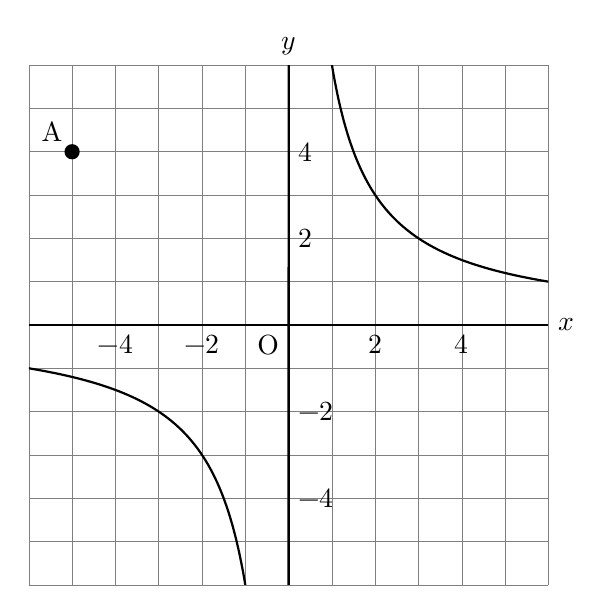
\begin{tikzpicture}[scale=0.55]
\draw[help lines] (-6,-6) grid (6,6);
\draw[thick](-6,0) -- (6,0)node[right]{$x$};
\draw[thick](0,-6) -- (0,6)node[above]{$y$};
\draw(0,0) node[below left]{O};
\foreach \x in {-4, -2, 2, 4} \draw ({\x},0) node[below]{$\x$};
\foreach \y in {-4, -2, 2, 4} \draw (0,{\y}) node[right]{$\y$};
\fill (-5,4) circle[radius=5pt] node[above left]{A};
\begin{scope}\clip(-6,-6) rectangle (6,6);
\draw [samples=100, smooth, thick, domain=-6:6] plot(\x, {6/\x});
\end{scope}
\end{tikzpicture}

\end{multicols}

\vfill

\noindent\fbox{\large\makebox[1em]{\text{\refstepcounter{kaunta}%
\arabic{kaunta}}}} \hspace{1pt}同じ種類のクリップがあります。クリップ全体の重さは$120\si{g}$でした。そのうち、12個を取り出してその重さをはかったら$18\si{g}$ありました。クリップは全部で何個ありますか。

%
\begin{flushright}%
\footnotesize{<知・技2点>}%
\end{flushright}%


\vfill

\newpage

\noindent\fbox{\large\makebox[1em]{\text{\refstepcounter{kaunta}%
\arabic{kaunta}}}} \hspace{1pt}ある車いすマラソンで、もっとも速い選手は分速$300\si{m}$、もっとも遅い選手は分速$120\si{m}$で走ります。下の図は横軸に時間、縦軸に距離をとって、もっとも速い選手ともっとも遅い選手の時間と進んだ距離をグラフにしたものです。

スタートしてから$6\si{km}$の地点で応援するとき、先頭の選手が通過してから何分後に、最後の選手が通過するでしょうか。また、なぜその答えになったのかをグラフを使って説明しなさい。ただし、選手は一定の速さで進むものとする。

%
\begin{flushright}%
\footnotesize{<知・技6点>}%
\end{flushright}%


\begin{center}
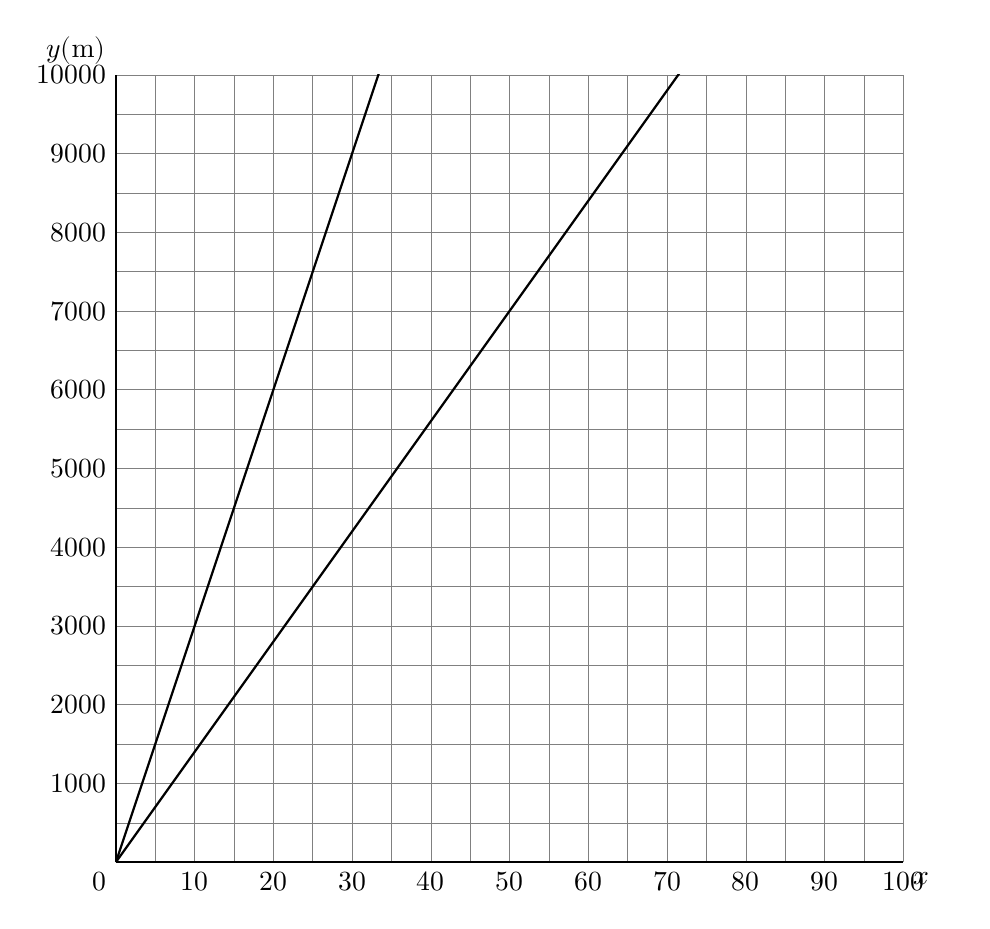
\begin{tikzpicture}[scale=0.5]
\draw[help lines] (0,0) grid (20,20);
\draw[thick](0,0) -- (20,0)node[below right]{$x\mbox{(分)}$};
\draw[thick](0,0) -- (0,20)node[above left]{$y(\si{m})$};
\draw(0,0) node[below left]{$0$};
\foreach \x in {1, 2, ..., 10} \draw ({2*\x},0) node[below]{$\x 0$};
\foreach \y in {1, 2, ..., 10} \draw (0,{2*\y}) node[left]{$\y 000$};
\draw ({20/3},20) node[above]{先頭の選手};
\draw ({100/7},20) node[above]{最後の選手};
\begin{scope}\clip(0,0) rectangle (20,20);
\draw[thick, domain=0:20] plot(\x, {3*\x});
\draw[thick, domain=0:20] plot(\x, {7*\x/5});
\end{scope}
\end{tikzpicture}

\end{center}

\setcounter{skaunta}{0}

\newpage

\noindent\fbox{\large\makebox[1em]{\text{\refstepcounter{kaunta}%
\arabic{kaunta}}}} \hspace{1pt}科学クラブでは、文化祭でスライム作りのイベントを行います。

%
\begin{flushright}%
\footnotesize{<思・判・表(1)3点、(2)5点>}%
\end{flushright}%


\begin{framed}
【スライムの作り方1人分の材料】

$\raise 0.2ex\hbox{\textcircled{\scriptsize{1}}}$\hspace{1em}大きめの容器に、ぬるま湯$100\si{ml}$とホウ砂$4\si{g}$を入れてよくかき混ぜる。

$\raise 0.2ex\hbox{\textcircled{\scriptsize{2}}}$\hspace{1em}$\raise 0.2ex\hbox{\textcircled{\scriptsize{1}}}$の容器に「のり」を$80\si{ml}$を加えて混ぜる。

$\raise 0.2ex\hbox{\textcircled{\scriptsize{3}}}$\hspace{1em}$\raise 0.2ex\hbox{\textcircled{\scriptsize{2}}}$の液体をかき混ぜると、「のり」がだんだんとかたくなってくる。
\end{framed}

(\text{\refstepcounter{skaunta}%
\arabic{skaunta}})\hspace{2.5pt}必要な材料を準備するとき、参加人数と必要な材料の量について、「$\underline{参加人数を決めると、それにともなって必要な材料の量がただ1つ決まる}$」という関係があります。

\hspace*{2em}下線部を、次のように表すとき、\fbox{\phantom{あああ}}に当てはまる言葉を書きなさい。

\begin{center}
\fbox{\phantom{材料の量}}は\fbox{\phantom{参加人数}}の関数である。
\end{center}

\vfill

(\text{\refstepcounter{skaunta}%
\arabic{skaunta}})\hspace{2.5pt}30人分の材料として、「のり」を$2400\si{ml}$用意しました。参加した人数で「のり」を等分して使い切るとき、1人分の「のり」の量と、人数は次のような関係になります。

\begin{center}
\fbox{(1人分の「のり」の量)$=$ $2400 \div$(人数) }
\end{center}


\hspace*{1em} イベント当日、40人が参加することになりました。人数が$\dfrac{4}{3}$倍になっていることから、当日の1人分の「のり」の量は、$80\si{ml}$を何倍すればよいかを考えます。何倍すればよいかを、次のア、イの中から1つ選び、記号で答えなさい。また、その理由を下の言葉のうちどれかを使って説明しなさい。

\begin{center}
\fbox{\hspace{3em} 関数 \hspace{3em} 比例 \hspace{3em} 反比例 \hspace{3em}}
\end{center}

\hspace*{1em} ア \hspace{1em} 1人分の「のり」の量を$\dfrac{4}{3}$倍にする。

\hspace*{1em} イ \hspace{1em} 1人分の「のり」の量を$\dfrac{3}{4}$倍にする。

\vfill

\end{flushleft}

\end{document}
